\chapter{Building LSP networks and describing the transmission dynamics of HPV on these networks}\label{ConstruccionYDinamica}

\section{Origin of the data}

%me enrollo un poco mas
Building a social network requires demographic data, for this model we have used data from the region of Valencia (Spain) that was collected from the Valencian Institute of Statistics (2013) \cite{IVE}, from this set of data we are interested in the distribution of males and females along with their age. The second set of data for this model has to do with sexual habits, this is the LSP for an individual, which was obtained from the Health and Sexual Habits Survey of 2003 \cite{INE}, and summarized in Tables \ref{tableLSPValues_men} and \ref{tableLSPValues_women}. 

\begin{table}[H]
	\centering
	\begin{tabular}{ccccccc}
		\multicolumn{7}{c}{MEN} \\
		\midrule 
		Age & $0$ LSP & $1$ LSP & $2$ LSP & $3-4$ LSP & $5-9$ LSP & $10+$ LSP \\
		\midrule
		14--29 & 0.107 & 0.207 & 0.131 & 0.225 & 0.168 & 0.162 \\
		30--39 & 0.027 & 0.225 & 0.128 & 0.21 & 0.17 & 0.24 \\
		40--65 & 0.019 & 0.268 & 0.14 & 0.193 & 0.163 & 0.217 \\
	\end{tabular} 
	\caption{Proportion of men per number of lifetime sexual partners (LSP) per age group. Note that the sum of the rows are 1.}
	\label{tableLSPValues_men} 
\end{table}

\begin{table}[H]
	\centering
	\begin{tabular}{ccccccc}
		\multicolumn{7}{c}{WOMEN} \\
		\midrule 
		Age & $0$ LSP & $1$ LSP & $2$ LSP & $3-4$ LSP & $5-9$ LSP & $10+$ LSP \\
		\midrule
		14--29 & 0.138 & 0.43 & 0.186 & 0.158 & 0.056 & 0.032 \\
		30--39 & 0.029 & 0.501 & 0.168 & 0.177 & 0.077 & 0.048 \\
		40--65 & 0.017 & 0.652 & 0.138 & 0.118 & 0.039 & 0.036 \\
	\end{tabular} 
	\caption{Proportion of wome per number of lifetime sexual partners (LSP) per age group. Note that the sum of the rows are 1.}
	\label{tableLSPValues_women} 
\end{table}

Some features of the distribution of contacts were: (i) the percentage of males and females with no partners is
very similar in each age-group; (ii) the proportion of women  with a single partner is, approximately, two times larger than men with only one partner; and (iii) the percentage of men with two or more partners is always larger than that of women except for women in the age-groups 14--29, and~30--39 in the case of two partners. The asymmetry in the behaviour of males and females should be taken into account in the construction of the network.

\section{Network model}

In this dissertation, we use the random network model as a basis to simulate the network of sexual contacts among individuals, but, in this model, the average number of connections depend upon the age-group as deduced from Tables \ref{tableLSPValues_men} and \ref{tableLSPValues_women}. A basic property of the network we are going to discuss is that the total number of LSP for the male population (M) must coincide with the total number of LSP for the female population (F). This is so because (in a purely heterosexual network) every link starting on a male must end in a female and viceversa. In mathematical terms:

\begin{equation}
\label{nodeseq}
\displaystyle\sum_{i=1}^M\, LSP_i=\displaystyle\sum_{j=1}^F\, LSP_j\; .
\end{equation}

About the estimation of sexual partners, there are some approaches to the number of LSP in males and females \cite{chandra2013sexual,mosher2005sexual} that are difficult to match. Generally speaking, males tend to overestimate the number of their sexual partners and females tend to underestimate it. Therefore, we considered the average LSP male value, $\left\langle k \right\rangle_m$, and calibrated the network so that results were consistent with data of Tables \ref{tableLSPValues_men} and \ref{tableLSPValues_women}, and estimated that the number of LSP in males in Spain was at least $4.5$. Networks with 100,000, 250,000, 500,000 and 750,000 have been used during the present study. It required a substantial computational power.

\section{Semi-Random Construction}
\label{subsec22}

From Table \ref{tableLSPValues_men} (proportion of male LSP aged 14--29), we have the following list:
$( 0.107, 0.314, 0.445, 0.67, 0.838, 1)$ for the accumulated proportion of males less than or equal to a given LSP number.
Now, we randomly generate a number $r$ between $0$ and $1$ and assign the number of contacts to every male node in the $14-29$
age group, in the network as follows:

\begin{itemize}[leftmargin=*,labelsep=5mm]
\item $r \le 0.107$ say that the corresponding male does not have an LSP,
\item $0.107 < r \le 0.314$ say that the corresponding male has one LSP,
\item $0.314 < r \le 0.445$ say that the corresponding male has two LSPs,
\item $0.445 < r \le 0.67$  say that the corresponding male has three or four LSPs uniformly distributed.
\item $0.67 < r \le < 0.838$ say that the corresponding male has five to nine LSPs uniformly distributed.
\item $0.838 < r \le 1$ say that the corresponding male has 10 or more LSPs.
\end{itemize}

Every node in the network is labelled by its gender and age randomly assigned according to the population histogram. The assignment of the number of bonds, as another label of the node, is not so straightforward since we must guarantee that the condition in Equation\ (\ref{nodeseq}) is verified. In~order to fulfill this condition, we take advantage of the uncertainty of statistics reports concerning individuals with $10$ or more LSPs.

Starting with the males, we assign the number of LSPs up to nine partners and, for $10$ or more partners proceed as follows: let $i_{\mbox{max}}$ be the number of males with nine or less partners. The unassigned males should be $M-i_{\mbox{max}}$ and the number of bonds that should be distributed among them is $M \left\langle k \right\rangle_m-\sum_{i=1}^{i_{\mbox{max}}}\, LSP_i$. By Euclidian division, this quantity can be expressed as $(M-i_{\mbox{max}}) n_m+r_m$, where $n_m \ge 10$. In our procedure, we assign a random number of bonds, uniformly distributed, in the interval $\left[10,2 n_m-10\right]$ to every male with $10$ or more LSPs, i.e.,
to~the $M-i_{\mbox{max}}$ unassigned males.

Now, we denote as $p_m$ the total number of bonds of the male population. We must take into account, as expressed in Equation\
(\ref{nodeseq}), that the total number of bonds of the female population should be the same. To impose that condition, we
proceed as follows: (i) assign the number of bonds to the females with nine or less partners following the statistical 
data in Tables \ref{tableLSPValues_men} and \ref{tableLSPValues_women}; (ii) the sum of all female LSPs in this group of $j_{\mbox{max}}$ members will be denoted by $s_f$. 
Then, $n_f=F-j_{\mbox{max}}$ is the number of females with $10$ or more LSPs; (iii) the number of bonds starting in the males and still unassigned to a female is $p_m-s_f= q_f n_f + r_f$, where $0 \le r_f < n_f$ and $n_f \ge 10$; (iv) we assign $q_f+1$ bonds to $r_f$ females still unassigned and $q_f$ bonds to the rest of $n_f-r_f$ females. The steps of this algorithm are also enumerated in the flow diagram in Figure  \ref{flux1}.

Notice that, for men and women with more than 10 LSPs, we assign their LSP in the most equitable way, assuming that all of them have, more or less, the same number of LSPs. Thus, we have a lot of hubs with a low number of contacts instead of a few hubs with a lot of contacts.

From the point of view of STD transmission, the latter situation leads to a faster transmission if the hub is infected, and, also, if the hub is vaccinated, the transmission is cut faster. Therefore, due to the lack of data about people with $10$ or more LSPs, we make the decision of being conservative in the transmission of the disease and in the effect of the vaccination campaigns.

Notice that this procedure implies that the condition in Equation\ (\ref{nodeseq}) is verified. After this procedure, we have obtained the following lists:
\begin{itemize}[leftmargin=*,labelsep=5mm]
\item $AgeMale\left[ i \right]$ is the age of the i-th male, $i=1,\ldots,M$,
\item $AgeFemale\left[ i\right]$ is the age of the i-th female, $i=1,\ldots,F$,
\item $kMale\left[ i \right]$ is the number of LSP for the i-th male, $i=1,\ldots,M$,
\item $kFemale\left[ i \right]$ is the number of LSP for the i-th female, $i=1,\ldots,F$.
\end{itemize}

These lists will be used to perform the connections of males and females and build the network. Note that, in Tables \ref{tableLSPValues_men} and \ref{tableLSPValues_women}, there are more females than males with few LSPs (comparing male and female percentages). It implies that there will be few women with a very large number of LSPs. This fact suggests us to start the assignment procedure with women with the largest LSPs. Otherwise, it would be possible that, when we have to assign LSPs of men to a female with a large number of LSPs, there~will not be enough men with free sexual partners to be assigned and, for this female, it would be impossible to satisfy the condition that the degree of each node was the number of its LSP. 

\begin{figure}[H]
	\centering
	\begin{tabular}{c}
		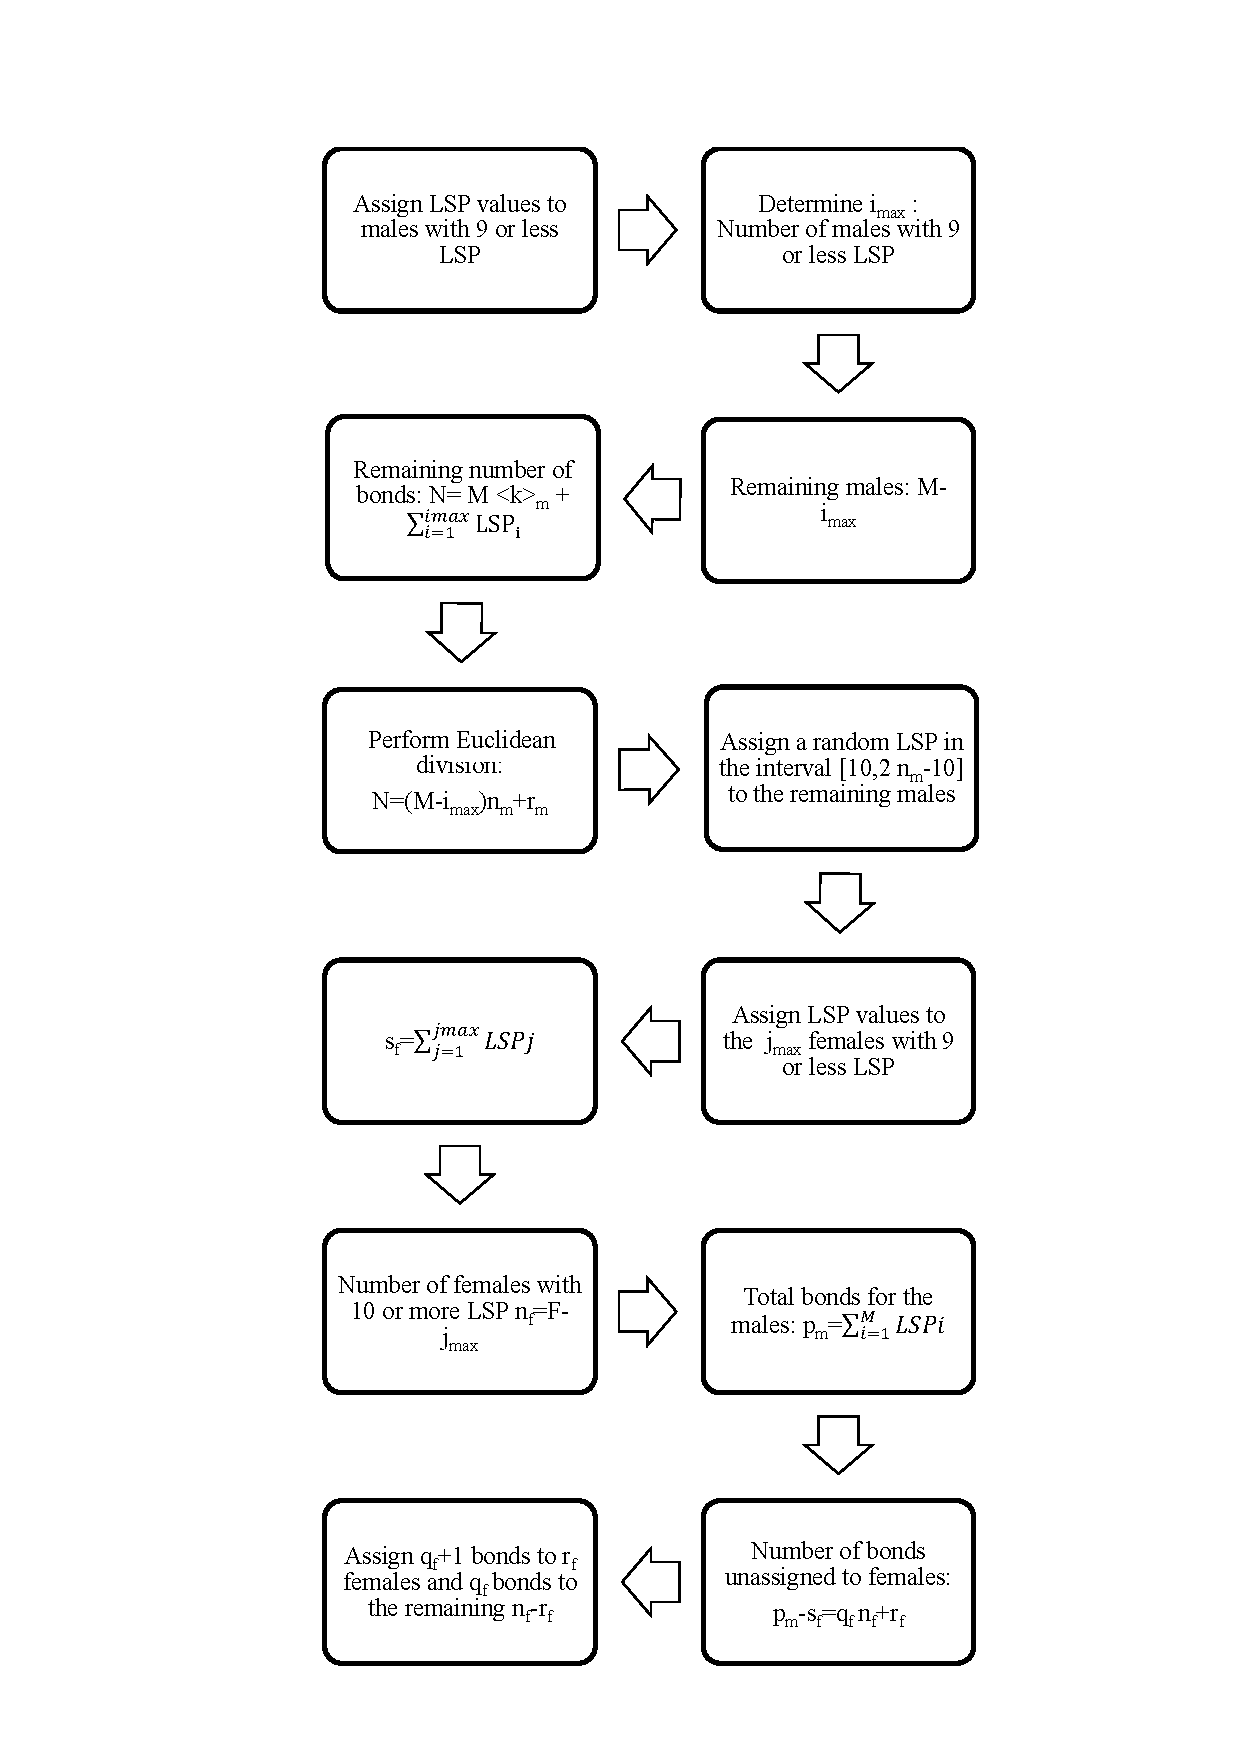
\includegraphics[width=\textwidth]{IMG/FluxDiagramI.pdf}
	\end{tabular}
	\caption{Flow diagram for the algorithm corresponding to the assignment of a number of LSPs to every male and female in the network.\label{flux1}}
\end{figure}

The assignment of partners was carried out by considering a principle of psychological similarity~\cite{gentner1997structure} or assortativity.
Hence, we are going to define a weight function assuming that: women with few LSPs usually match men with few LSPs; people with four or more LSPs use to join with people with four or more LSPs; and couples where one of them has a large number of LSPs and the other few LSPs will be uncommon. Then, for the woman $i$ and the man $j$, we define the following weight~function:

\begin{equation}
\pi(i,j) = 
\begin{array}{l}
\left\lbrace \begin{array}{lc}
| kFemale[i] - kMale[j] | & kFemale[i], kMale[j] \le 4 \\
0 & kFemale[i], kMale[j] > 4 \\
100 & \mbox{otherwise}
\end{array} \right\rbrace, \\
\\
 + | AgeFemale[i] - AgeMale[j] - 1.8 |.
\end{array}
\label{peso}
\end{equation}

The combined weight function, which takes into account the age difference of the partners, $\vert AgeFemale[i] - AgeMale[j] - 1.8 \vert$ is defined in this way because some studies show that the average age difference among the members of a couple in Spain is $1.8$ years \cite{miret2010similitud}. 

%The MSM population (around $3.88$ \% of the total male population in Spain)\cite{INE} can also be incorporated into the model, but, in this subpopulation, the connectivity would be larger than the heterosexual network. The MSM population would also be connected with the heterosexual one by links with women in such a way that every MSM individual has a link with a woman with five or more contacts \cite{acedo2017calibrating}.

The estimated percentage of men who have sex with men (MSM) is $3.88\%$  \cite{INE}. The situation for the MSM population is different of the one shown in Tables \ref{tableLSPValues_men} and \ref{tableLSPValues_women}, because the average number of sexual partners is estimated in 39 regardless of age, but this number increases with age with a peak of 59 in the 40-49 age-group \cite{Durex2002}.
A difficulty arises because we have little information about the number of sexual contacts of women who have sex with women (WSW) subpopulation. In a personal communication by Dr. Mireia D\'iaz from the Catalan Institute of Oncology (IDIBELL) we were informed that HPV hardly spreads among WSW, and almost all MSM, sometimes in their lives, had a woman partner. Consequently, we have simulated these connections by assigning a contact to every man in the MSM subpopulation with woman with 5 partners or more. This is done according to the assortativity principle, that is, people use to join with people with similar habits.

The assignment of links is then performed by the Greedy Randomized Adaptive Search Procedure (GRASP) algorithm \cite{cormen2009introduction,feo1995greedy}. %Details about the construction of the whole network have been provided in previous studies \cite{acedo2017calibrating,BuildingLSPNova}. 

